\chapter{Introduction}

\section{Motivation}
% Search is amazing, ability to reason given limitied information, we can do many things without
% fully observing our environment. 
% Examples where partial observability is everywhere in the world and how we as humans have to deal 
% with it on a day to day basis which almost second nature to use. We do not have to think about it, we 
% just do it. This is increadibly difficult to do for robots, acting and reasing given incomplete information
% is one of the most challanging aspects of artificel intiellegence. Because of the sheer branching factor. 
% 
% Neuroscience evidence 
%
% Long-term and short term memory
%
%
% When reasoning with respect to uncertainty, number of assumptions are made
%

%
% 1) Describe uncertainty & risk in the world how important it is for biological entities to approprietly take it 
%    into account for survivial.  
%
%    Description of what humans are able to do on a day to day basis and how important uncertainty is Balancing risk.
%    Evidence of humans being expectation maximisers.
%
% 2) 
%

% An action is the result of two hidden states; Our beliefs and desires.

%
% 3) How is uncertainty handles in artificel intelligence ?
%
%
%
% 4) Uncertainty in robotics; how is it handled.
%
%
% 5) Summary

% 1)
Taking long term decisions or spontaneous reactive actions when presented with incomplete information or partial knowledge is 
paramount to the survival of any biological or synthetic entity. Reasoning given uncertainty is a continuously occurring event throughout our 
livelihood. When considering long term decisions an abundance of examples come to mind; for instance in economic investments 
uncertainty is to the best of efforts quantified and minimised such to avoid unwarranted risks. Reactive actions are just as common; 
when looking for the snooze button of an alarm clock, early in the morning, our hand seems to autonomously search the surrounding space picking up
sensory cues gradually acquiring information guiding us towards the button. All the above types of decisions require the integration of 
evidence and an ability to predict the outcomes of the taken decisions such to insure a favourable end state. 
Abilities close to these have met mixed levels of success in Artificial Intelligence (AI) \& robotics. There is a been 
noticeable success in artificial agents beating humans at board games (backgammon, chess and go) but having a robot successfully 
climb a staircase, open a door or pick up a glass are still ongoing open problems. 

It is not yet fully understood how decisions are taken, yet alone under uncertainty. The difficulty is that two processes responsible 
for the synthesis of our actions and decisions, our beliefs and desires, are not directly or easily measurable. There is growing interest in 
Neuroscience to understand the mechanisms underlying perception and decision making under uncertainty \cite{decision_un_2013}; there is not 
yet a consensus on the biological mechanisms involved in decision making and efforts are 
ongoing\footnote{the human brain project: https://www.humanbrainproject.eu/} to construct plausible models of our decision processes. 
At a higher level, early efforts to modelling human decision making was in mathematics \& economics 
(\cite{Bernoulli1954},\cite{VonNeumann1944}), in which gambles and investments were chiefly considered. There has been 
considerable effort in many fields (neuroscience, cognitive science, physiology, economics, etc..) to understand how decisions and actions 
are taken from the role of our neurons too high level decision like gambles, orientation and navigation problems to reflexes. 
 
% . In locomotion behaviour uncertainty plays a role on how we plan our paths, there is evidence 
%in Neuroscience that the hypocampus plays an important role our internal representation.

% Understanding and subsequently predicting the way we reason 
% with respect to uncertainty and de facto how we handle risk has been modelled by a utility function and the probabilistic outcome 
% of our decisionse

% Should speak about evidence of neuroscience activity during locomotion. Do we know which parts of the brain are being 
% triggered when we are doing search. Is there neuroscience evidence of an internal map representation in our brain 
% ego-centric allocentric represenation (
 
% 3) Aritficiel intelligence & robots (How is uncertainty taken into account in the decision process)

Artificial intelligence \& robotics considered early on uncertainty in decision making, 
where the predominant domain of application was spatial navigation, \cite{ActingUncertainty_1996}. The problem is composed 
into of two parts: the construction and representation of a world model (the map) and a planner which can reason with 
respect to this model such to accomplish an objective. The world construction problem attracted a large amount of 
research with many successfully applications in a wide spectrum of robotic domains (AUV, UAV, etc..). The integration of mapping 
with planning in a single framework is still difficult to achieve and is based on either representing the decision problem as a 
Partially Observable Markov Decision Process (POMDP) which are notoriously difficult to solve for large scale problems, or through search heuristics.  
The mapping problem can generally be solved when assuming the uncertainty is Gaussian and thus quantifiable 
by a few parameters and the uncertainty originates from the imprecision of the sensors.

%As for the planning problem solutions are feasible
%under the restrictive assumption of a discretization of the world, observations and actions of the robot. As a result there are very
%few examples where uncertainty is considered in an optimal decision make process when considering a continuous state, action 
%and observation space.

\begin{figure}
 \centering
 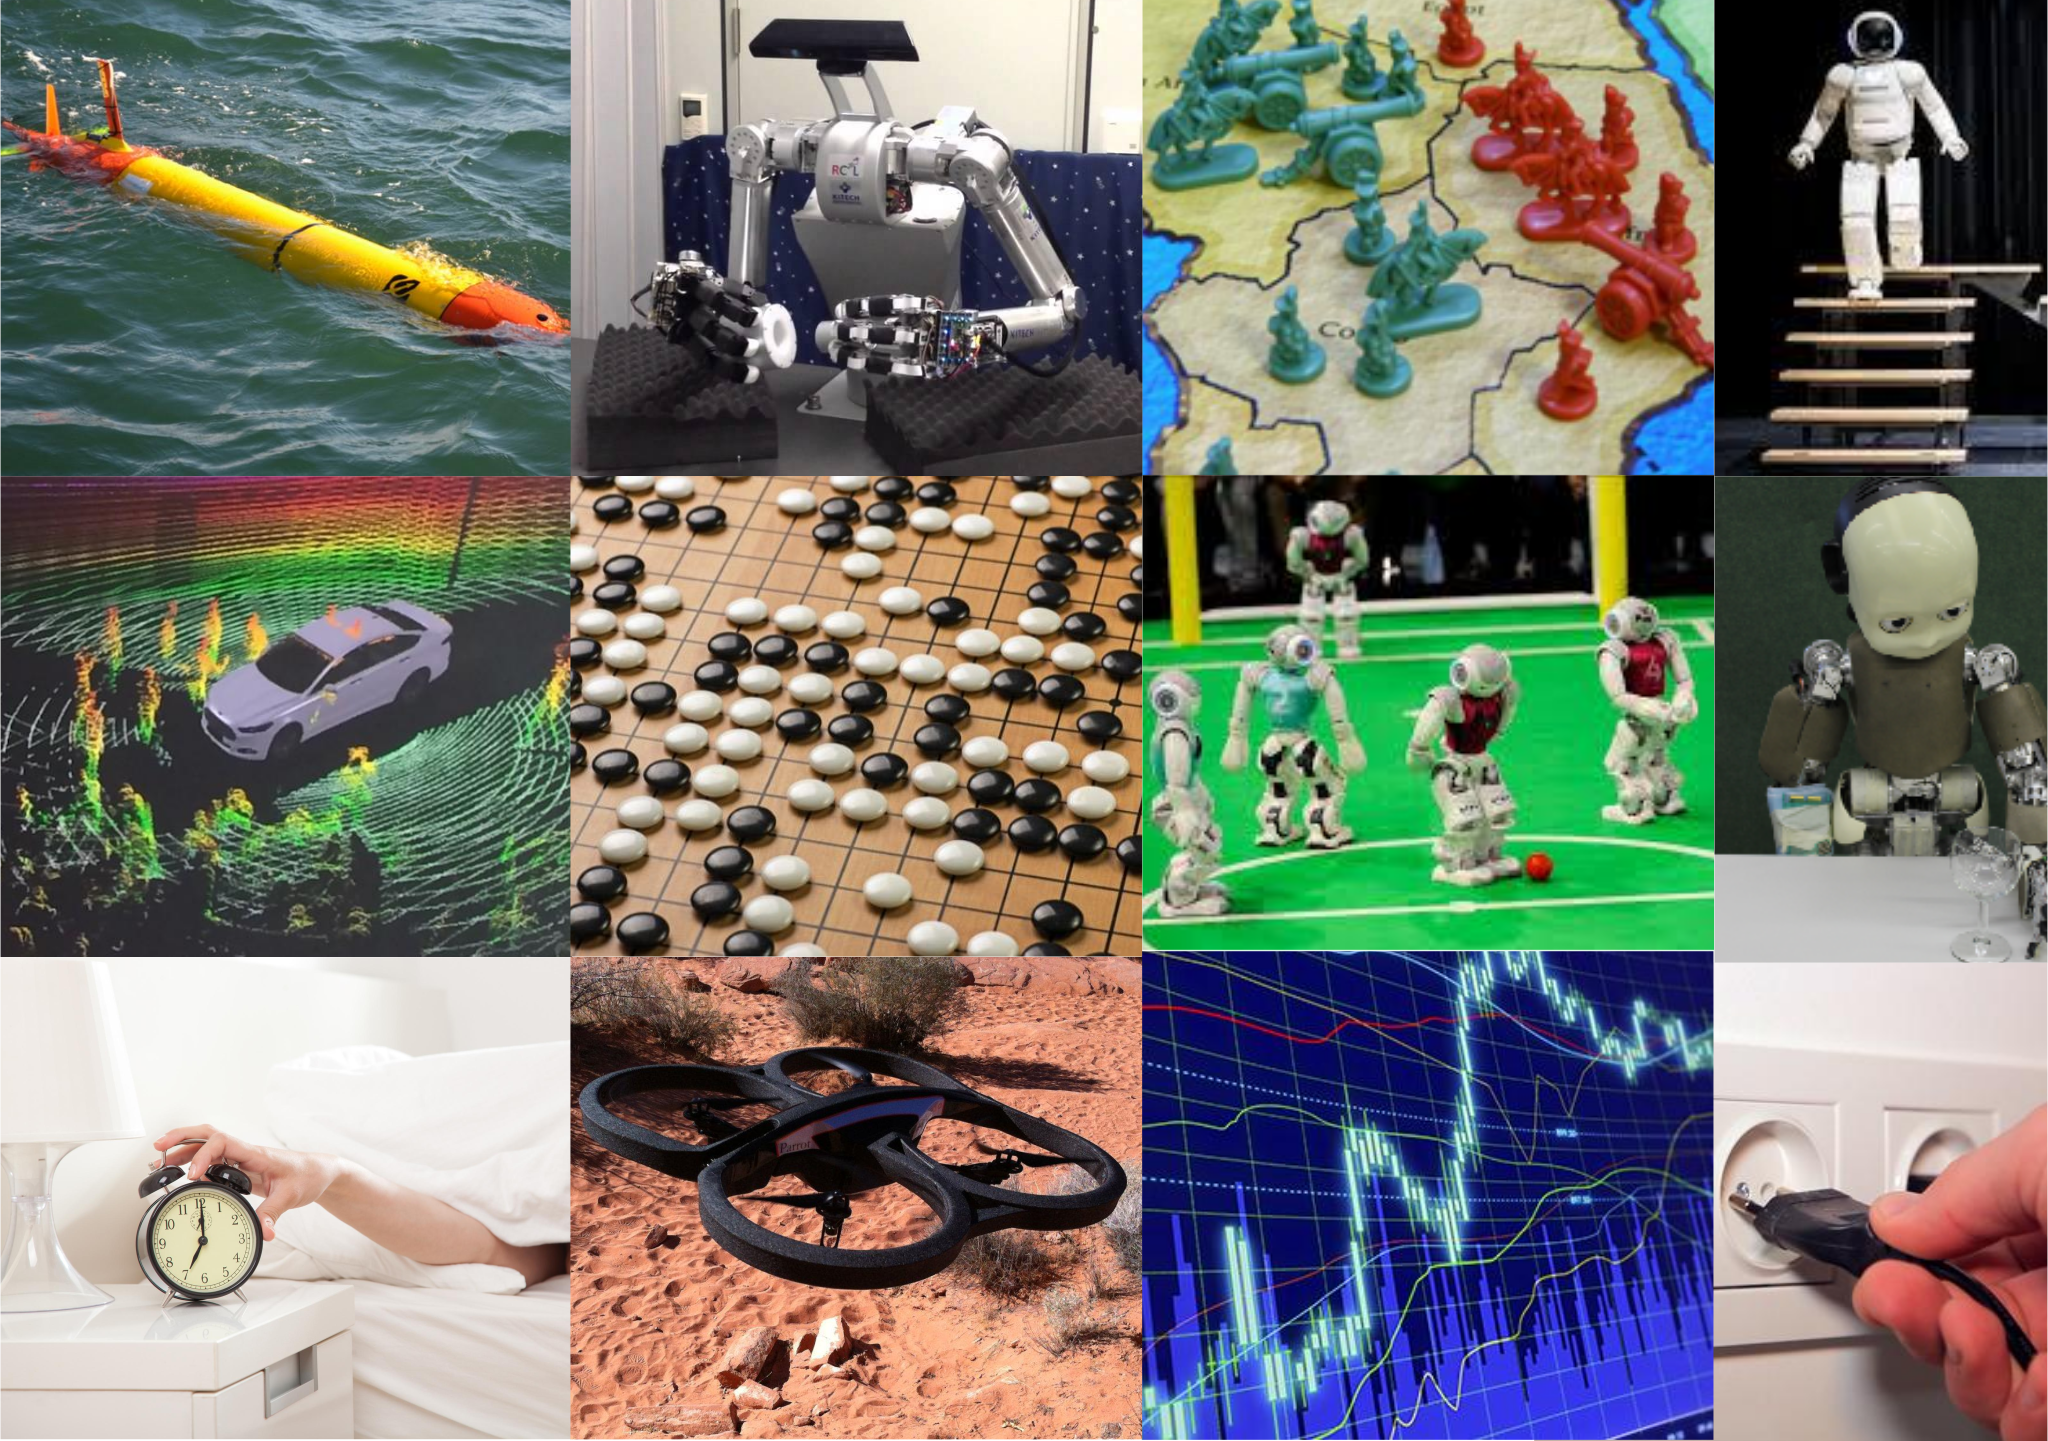
\includegraphics[width=0.9\textwidth]{examples.pdf}
 \caption{Examples of the decision making under uncertainty in both robotics and everyday life situations. Images taken from the public domain.}
\end{figure}

In summary there are still open problems in decision making when considering partial observability, whilst 
the mapping problem has been studied under a constraining set of assumptions. In this thesis we address both problems 
under extreme levels of uncertainty. 
For the decision making side we leverage humans foresight and reasoning in a Learning from Demonstration (LfD) (\cite{Billard08chapter})
framework, which is used to transfer skills from an expert teacher (usually a human) to a robot. Examples include the transfer of 
kinematic task constraints, stiffness and impedance constraints and motion primitives, just to name a few.
It has been shown, for the moment being, both humans and animals are far better at navigation than robots especially when 
uncertainty is present (\cite{stankiewicz2006lost}). For the mapping problem we develop a Bayesian filter which is non-parametric 
and has no explicit representation of a joint distribution.



%The advantage of taking a LfD approach and encoding the demonstrated behaviour in a asynchronous dynamical system (ADS) is that we have robustness to perturbation
% and a generalisation over the entire state space. 

\section{Contribution}
% - One page 1/2 

In this thesis we bring to light two main ideas. The first is the transfer of human behaviour to robots
in tasks where a lot of uncertainty in present, making them difficult to solve using traditional techniques.
The second is a non-parametric Bayesian state space filter which is efficient under sparse sensory information 
and high levels of uncertainty.

Throughout the work in this thesis we consider case studies in which vision is not available, leaving tactile and 
haptic information. This choice was made to induce a high level of uncertainty making it easier to study its effect 
on the decision making process. As a consequence the tasks we consider are by nature, haptic and tactile searches.
We detail next in the following three sections the contributions of this thesis.

\subsection{Learning to reason with uncertainty as humans}

A Markov Decision Process (MDP) allows to formulate a decision problem in terms of states, actions, a discount factor 
and a cost function. Given this formulation and a suitable optimisation method (dynamic programming, temporal difference, etc..) 
a set of optimal decision rules are returned, known as a policy. The benefit of this approach 
is that the policy is non-myopic and sequences of complicated actions can be synthesised to achieve a goal which 
an opportunistic policy would fail to achieve. A Partially Observable Markov Decision Process (POMDP), is 
a generalisation of an MDP to a hidden state space and only observation are available relating 
to the state space. Finding an exact optimal solutions to a POMDP problem is notoriously difficult due to 
the computational complexities involved. Sampled based approaches to solve a POMDPs relay heavily on a 
a good trade off between exploration and exploitation actions. Good explorative actions allow to discover 
the set of optimal decisions/actions.

%An exact solution to a POMDP is only feasible in simple toy problems 
%(\cite{Thrun_Burgard_Fox_2005}) and existing approximate solutions are tailored for discretized 
%representation of states, actions and observations and an optimal solution heavily relies on 
%the exploration-exploitation trade-off.

In this thesis we propose a Learning from Demonstration approach to solving POMDP problems in
haptic and tactile search tasks. Our hypothesis is that if we know the mental state of the human 
expert in terms of his believed location and observe his actions we can learn a statistical policy 
which mimics his behaviour. Since the human's beliefs are not directly observable we infer them 
by assuming that the way we integrate evidence is similar to a Bayesian filter. There is   
evidence both in cognitive and neuroscience that this is the case (\cite{Bake_Saxe_Tene_2011}). From 
the expert human demonstrations of the task we learn a cognitive model of the humans decision process 
by learning a generative joint distribution over his beliefs and actions. The generative distribution 
is then used as a control policy. By this approach we are able to have a policy which can handle uncertainty
similarly to humans. 

\subsection{Non-parametric Bayesian state space filter}

Simultaneous Localisation and Mapping (SLAM) is concerned with the development of filters to accurately and efficiently infer 
the state parameters (position, orientation,...) of an agent and aspects of its environment, commonly referred to as the map. 
It is necessary for the agent to achieve situatedness which is a precondition to planning and reasoning. The 
predominant usage of SLAM algorithm make the assumption that uncertainty is related to the noise in the sensor measurements. In 
our haptic search tasks there is no visual information and a very large amount of uncertainty. Most of the sensory
feedback is negative information, a term used to denote the non event of a sensor response from the objects in question.
In the absence of recurrent sightings or direct measurements of objects there are no correlations from the measurement errors 
which can be exploited. 

In this thesis we propose a new SLAM filter, which we name Measurement Likelihood Memory Filter (MLMF), in 
which no assumptions are taken with respect to the shape of the uncertainty (it can be Gaussian, multi-modal, uniform, etc..) and 
motion noise. From these loose assumptions, we adopt a histogram parametrisation (this is considered non-parametric 
because a change in a parameter has a local effect). The conceptual difference between the MLMF and standard SLAM filters, 
such as the Extended Kalman Filter (EKF), is that we avoid representing the joint distribution since it would entail a shattering space and time complexity. 
This is achieved by keeping track of the history of measurement likelihood functions. We demonstrate that our approach gives 
the same filtered marginals as a histogram filter. In such a way we achieve a Bayes filter which has both linear space and 
time complexity. This filter is well suited to tasks where the landmarks are not directly observable.

\subsection{Reinforcement learning in belief space}

We propose a Reinforcement Learning framework for the task of searching and connection a power plug to a socket, with only haptic 
and tactile information. We previously addressed this setup by learning a generative model of the beliefs and actions with data 
provide by human demonstrations following the LfD approach. However, it is usually the requirement that 
the teach is an expert, with few notable exceptions (\cite{rai2013learning}). Since we were solely learning a 
statistical controller, bad and good demonstrations will be mixed in together. By introducing a cost function 
representing the task we can explicitly have a quality metric of the provided demonstrations. In this way 
we can optimise the parameters of our generative model to maximise the cost function. In this LfD Reinforcement 
Learning setup with a very simple cost function we can have a significant improvement of our a policy.

\section{Thesis outline}

The thesis is structured accordingly to the three main contributions outlined in the previous section, 
and all will have their individual chapter. We outline below the structure of the thesis.

\begin{minipage}[c]{0.9\textwidth}
\paragraph{Chapter 2 - Background}\\
In this chapter we introduce and mathematically formalise the sequential decision making problem 
under uncertainty and we provide a detailed literature review of the related work in this domain.
We provide a brief introduction to \textit{Decision Theory} before focusing on the work 
in AI \& robotics relevant to POMDPs whilst highlight their relevance and contribution to our work. 
\end{minipage}

\begin{minipage}[c]{0.9\textwidth}
\paragraph{Chapter 3 - Learning to reason with uncertainty as humans}\\
In this chapter we present an approach for transferring human skills in a blind haptic 
search task to a robot. The belief of the human is represented by a particle filter and 
all subsequent beliefs are inferred from the humans motions provided via a motion tracking
system. A generative model of the joint belief and actions distribution is learned and used
to reproduce the behaviour on a WAM and KUKA robot in two search tasks. Experimental 
evaluations showed the approach to be superior to greedy opportunistic policies and traditional
path planning algorithms. The major parts of this chapter have been presented \cite{Chambrier2014}.
We also provide a review of work related to humans taking decisions under uncertainty 
in spatial navigation and haptic tasks with an emphasis on works which consider diminished or no 
visual information. 
\end{minipage}


\begin{minipage}[c]{0.9\textwidth}
\paragraph{Chapter 4 - Non-parametric Bayesian state space filter}\\
In this chapter we present approach to perform a state space estimation of a map and agent 
given that there is no direct observation between the landmarks and agent. We demonstrate that 
by not explicitly parametrizing the full joint distribution of the landmarks and agent but instead
keeping track of the applied measurement functions we can fully reconstruct the optimal Bayesian 
state estimation. The advantage of our approach is that the space complexity is linear as oppose 
to exponential. We validate our approach in 2D search navigation tasks. This work is currently under review.
We also given a overview of the literature of SLAM and emphasis the position of our filter within it.
\end{minipage}

\begin{minipage}[c]{0.9\textwidth}
\paragraph{Chapter 5 - Reinforcement learning in belief space}\\
In this chapter we present an approach similar to the one presented in chapter 3 with the difference that
we explicitly encode the task through the introduction of a binary objective function and we consider a peg-in-hole
task under high levels of uncertainty. The task requires both high and low levels or precision to be able to accomplish it,
which makes it particularly interesting. We learn a value function approximation of the belief space through locally weighted 
regression and approximate dynamical programming.
By combining a LfD approach in this Actor-critic Reinforcement Learning framework, we demonstrate an improvement upon 
a purely statistical controller with nearly no additional cost. 
We additionally provide a review of RL methods in the context of POMDPs.
\end{minipage}

\begin{minipage}[c]{0.9\textwidth}
\paragraph{Chapter 6 - Conclusion}\\
We conclude by providing a holistic summary of our work and achievements. We draw attention to the current 
open problems and directions for future work in field of uncertainty and reasoning in Artificial intelligence and robotics.
\end{minipage}







